\section{Strahlungsprozesse der Erde}
\note{
  \begin{itemize}
    \item[] Zentrale Frage: Was bestimmt das Klima?
    \item[] Wie ist ein Erdklima möglich?
    \item[] Grundlage bildet die Sonne. Aber was ist der Unterschied zu unseren Nachbarn?
    \item[] Mittlere Oberflächentemperaturen: Venus \SI{464}{°C}, Mars \SI{-55}{°C}
    \item[$\rightarrow$] Die Erde hat eine Atmosphäre
    \item[] Die Atmosphäre sorgt dafür, dass eine gewisse Menge der Sonnenenergie auf der Erde verbleibt
    \item[] lebenfreundliche Temperaturen werden auf der Erde erreicht
  \end{itemize}
}
%\begin{frame}
%  \frametitle{Strahlungsprozesse der Erde}
%  %TODO
%\end{frame}

\begin{frame}
	\frametitle{Aufbau der Atmosphäre}
	\begin{figure}
		\centering
		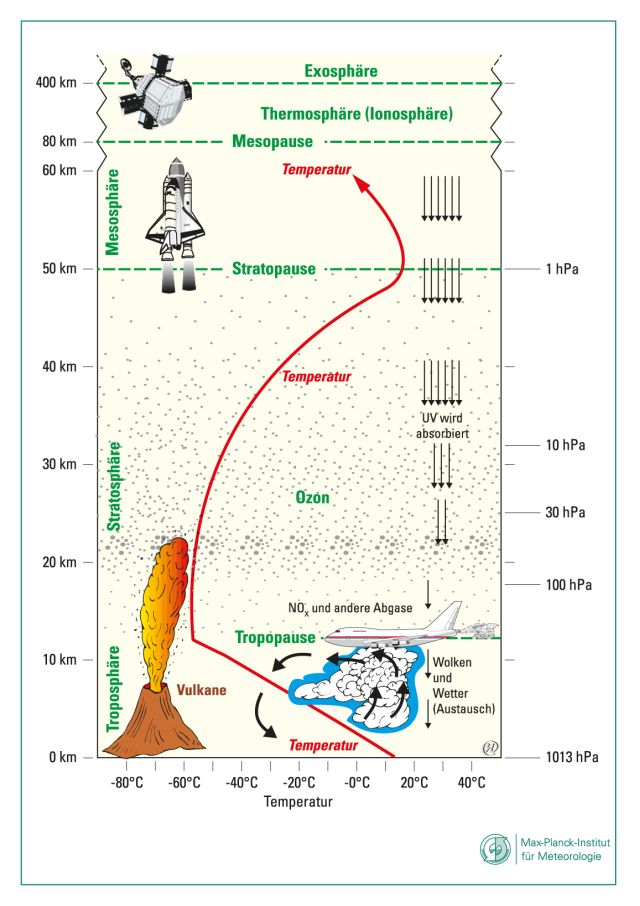
\includegraphics{bilder/atmosphaere-stockwerkaufbau_bildungsserver_hh.jpg}
		\caption{Schematischer Aufbau der Atmosphäre, Quelle: Bildungsserver Hamburg}
	\end{figure}

  \note{
  \begin{itemize}
    \item[] Troposphäre, \SIrange{10}{12}{km}
    \begin{itemize}
      \item[] \SI{80}{\%} der Atmosphärenmasse, enthält fast allen Wasserdampf
      \item[] Hier finden alle wetterrelevanten Phänomene statt
      \item[] ersten \SIrange{1}{2,5}{km} starker Einfluss der Erdoberfläche
      \item[] Jetstreams an oberer Grenze, kein Transport von H$_2$0 von Troposphäre in die Stratosphäre
    \end{itemize}
    \item[] Stratosphäre, \SIrange{12}{50}{km}
    \begin{itemize}
      \item[] Anstieg der Ozonkonzentration sorgt für Temperaturanstieg
      \item[] Die Prozesse hier (Strahlung, Dynamik, Chemie) relevant für Klima in der Troposphäre
    \end{itemize}
    \item[] Mesosphäre, \SIrange{50}{80}{km}
    \begin{itemize}
      \item[] Stetige Temperaturabnahme
    \end{itemize}
    \item[] Thermosphäre, \SIrange{80}{400}{km}
    \begin{itemize}
      \item[] extrem geringe Teilchendichte, Weltram fängt bei \SI{100}{km} an (NASA), Bremswirkung der Atmosphäre aber auch bei \SI{400}{km} Höhe noch spührbar (ISS wird regelmäßig von andockenden Raumschiffen auf ihre Bahn zurück geschoben)
    \end{itemize}
    \item[] Exosphäre, \SIrange{400}{1000}{km}
    \begin{itemize}
      \item[] quasi Vakuum
    \end{itemize}
    \item[] Grenzen nicht hart, Troposphäre z.B.
    \begin{itemize}
      \item[] 10-12 km im Durchschnitt
      \item[] 8 km an den Polen
      \item[] 17-18 km in den Tropen
    \end{itemize}
  \end{itemize}
  }
\end{frame}

%Übergang: Ohne die Atmosphäre hätten wir auf der Erde eine durchschnittliche Temperatur von -18 Grad, durch die Atmosphäre und die atmosphärischen Gase ist es aber im Mittel etwa etwa 35 Grad wärmer -> 15 Grad

\begin{frame}
  \frametitle{Strahlungshaushalt}

  \begin{figure}
  	\centering
    \begin{tikzpicture}
      \node[anchor=south west,inner sep=0] (image) at (0,0){
  	   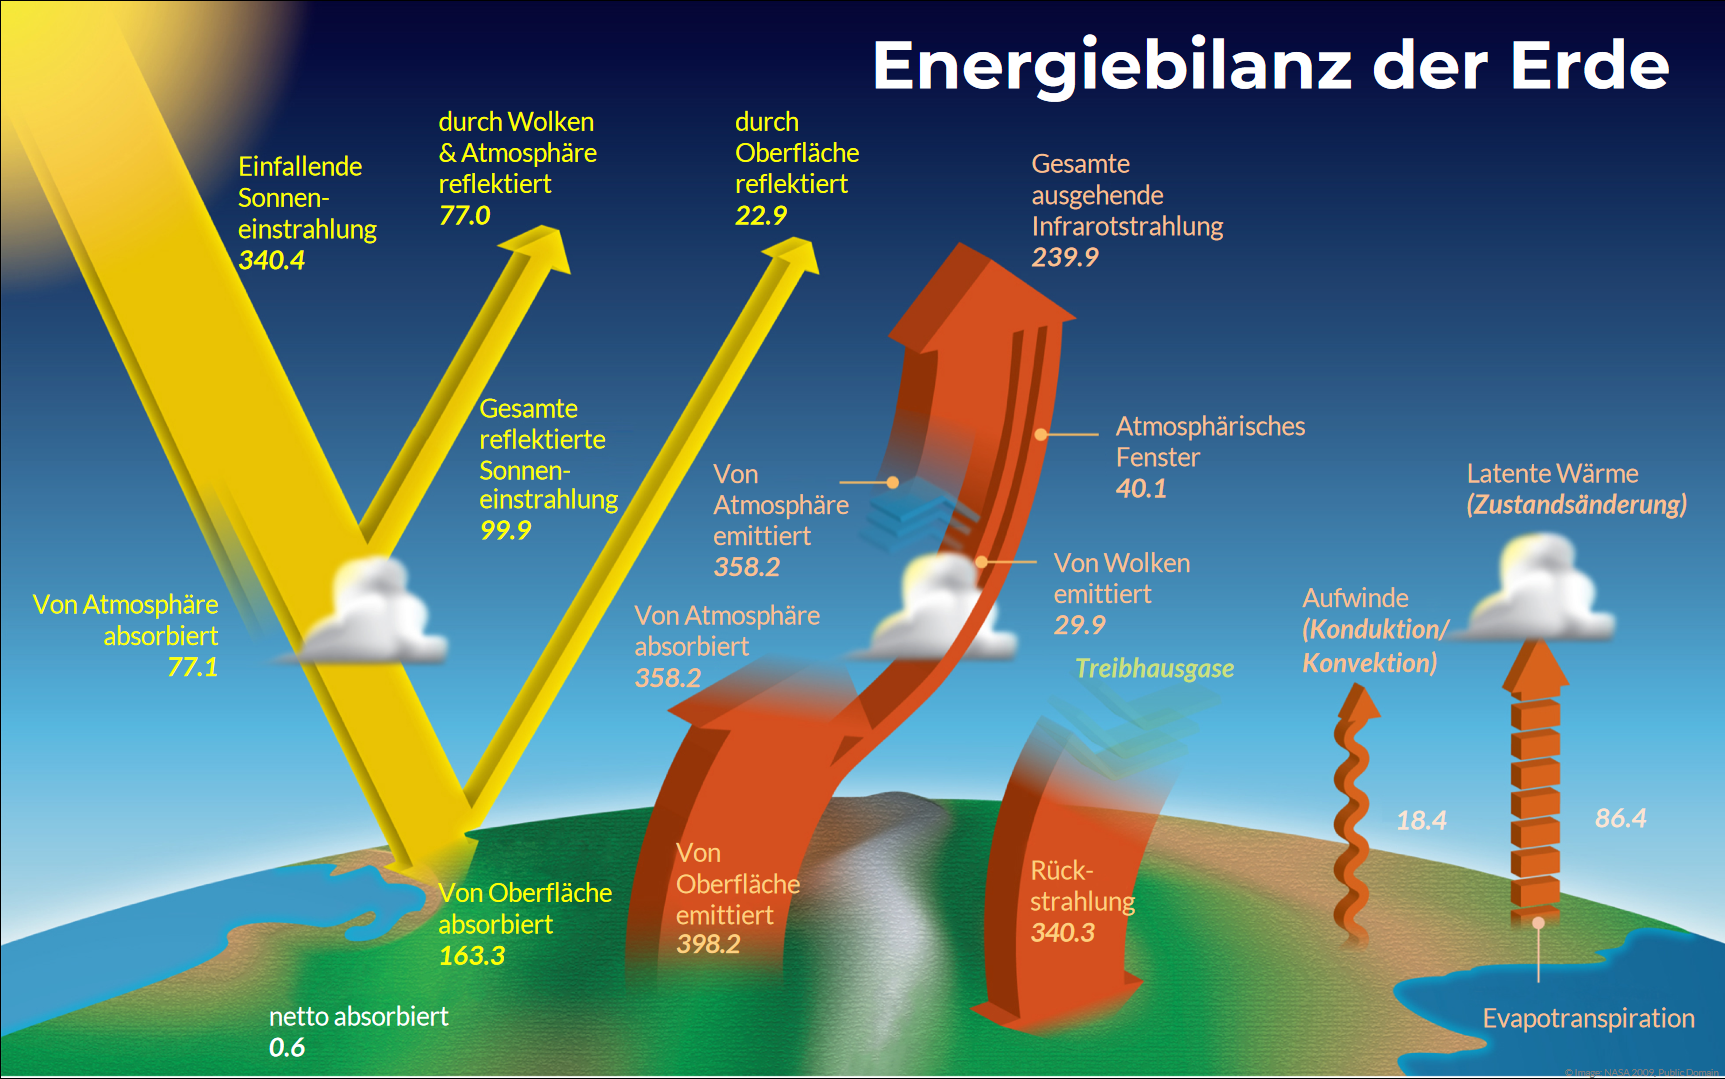
\includegraphics[width=0.8\linewidth]{bilder/Energiebilanz_der_Erde_NASA.png}};
      \uncover<2->{
        \node[anchor=south west, text=red] (text) at (4.7, 3.235) {\scriptsize\textbf{\rule[0.5ex]{2em}{0.55pt}\;\num{169.9}}};
      }
    \end{tikzpicture}
  	\caption{Strahlungshaushalt der Erde, Angaben in W/m$^2$, Quelle: NASA nach Kiehl und Trenberth 1997, Übersetzung: S4F} % Die Abbildung ist in den Folien der S4F Vertiefung zum Klimawandel (S.21) aber dort leider nur spärlich referenziert. Annahme: Jemand der S4F hat dieses Bild Übersetzt und dem Abbildungs-Pool hinzugefügt.
  \end{figure}

  %Abbildung für Strahlungshaushalt einfügen z.B: vom Bildungsserver Hamburg https://bildungsserver.hamburg.de/atmosphaere-und-treibhauseffekt/2069644/atmosphaere-strahlungshaushalt-artikel/
  % bzw. vom den S4F materialien: http://files.scientists4future.org/Themen/2.%20Klimawandel/Als%20PDFs/S4F-03%20Klima%20Vertiefung%202020-01-31.pdf
  % oder vom IPCC AR5 Figure 2.11
  \note{
  \begin{itemize}
    \item[] Ohne die Atmosphäre hätten wir eine durchschnittliche Oberflächentemperatur von \SI{-18}{°C}
    \item[] Mit Atmosphäre (Treibhausgase) ist es im Mittel \SI{33}{°C} wärmer, wir haben eine durchschnittliche Oberflächentemperatur von \SI{15}{°C}
    \item[] Solarkonstante: \SI{1368}{W\per m\squared} oberhalb der Atmosphäre
    \begin{itemize}
      \item[] Zur Erwärmung der Atmosphäre verfügbar: \SI{340}{W\per m\squared} auf Grund der Kugelgestalt und der Nachtseite der Erde
      \item[] rund \SI{70}{\%} der gesamten einfallenden Strahlung werden absorbiert (Atmosphäre (\SI{22}{\%}), Oberfläche (\SI{48}{\%}))
      \item[] rund \SI{30}{\%} der gesamten einfallenden Strahlung werden reflektiert (Wolken und Atmosphäre (\SI{23}{\%}), Erdoberfläche (\SI{7}{\%}))
    \end{itemize}
    \item[] Damit sich die Erde nicht aufheizt, muss die absorbierte Energie wieder abgegeben werden
    \item[$\rightarrow$] Die absorbierte kurzwellige Sonneneinstrahlung wird als langwellige infrarot Strahlung wieder abgegeben (vgl. Eingehend \SI{340}{W\per m\squared} und Ausgehend \SI{100}{W\per m\squared} reflektiert, sowie \SI{240}{W\per m\squared} als IR abgestrahlt)
    \item[] Zusätzlich \SI{340}{W\per m\squared} Rückstrahlung $\rightarrow$ Woher kommen die?
    \begin{itemize}
      \item[] Einergiebilanz der Atmosphäre: \SI{77}{W\per m\squared} Sonneneinstrahlung + \SI{358}{W\per m\squared} Erdeinstrahlung + \SI{18}{W\per m\squared} Aufwinde + \SI{86}{W\per m\squared} latente Wärme - \SI{200}{W\per m\squared} von Wolken und Atmosphäre emittiert = \SI{340}{W\per m\squared} bleiben übrig
      \item[$\rightarrow$] Treibhauseffekt
    \end{itemize}
  \end{itemize}
  }
\end{frame}

% Fokus auf den Treibhauseffekt, d.h. vorherige Abbildung reduziert um ein paar Energieflüsse  (mitte)
% zB Sonneneinstrahlung- Atmosphärische Reflexion = 235 W/m2
% Die Abbildung zeigt zum einen die Temperatur auf der Erde ohne die Strahlungsbilanz der Erde(links) außerdem nochmal den atmosphärischen Aufbau (rechts)
% In der Mitte ist die Auswirkung der Treibhausgase zu sehen

\begin{frame}
  \frametitle{Treibhauseffekt}
  \begin{figure}
  	\centering
    %TODO Bild austauschen, besser Absorption von Treibhausgasen
    \only<1>{
  	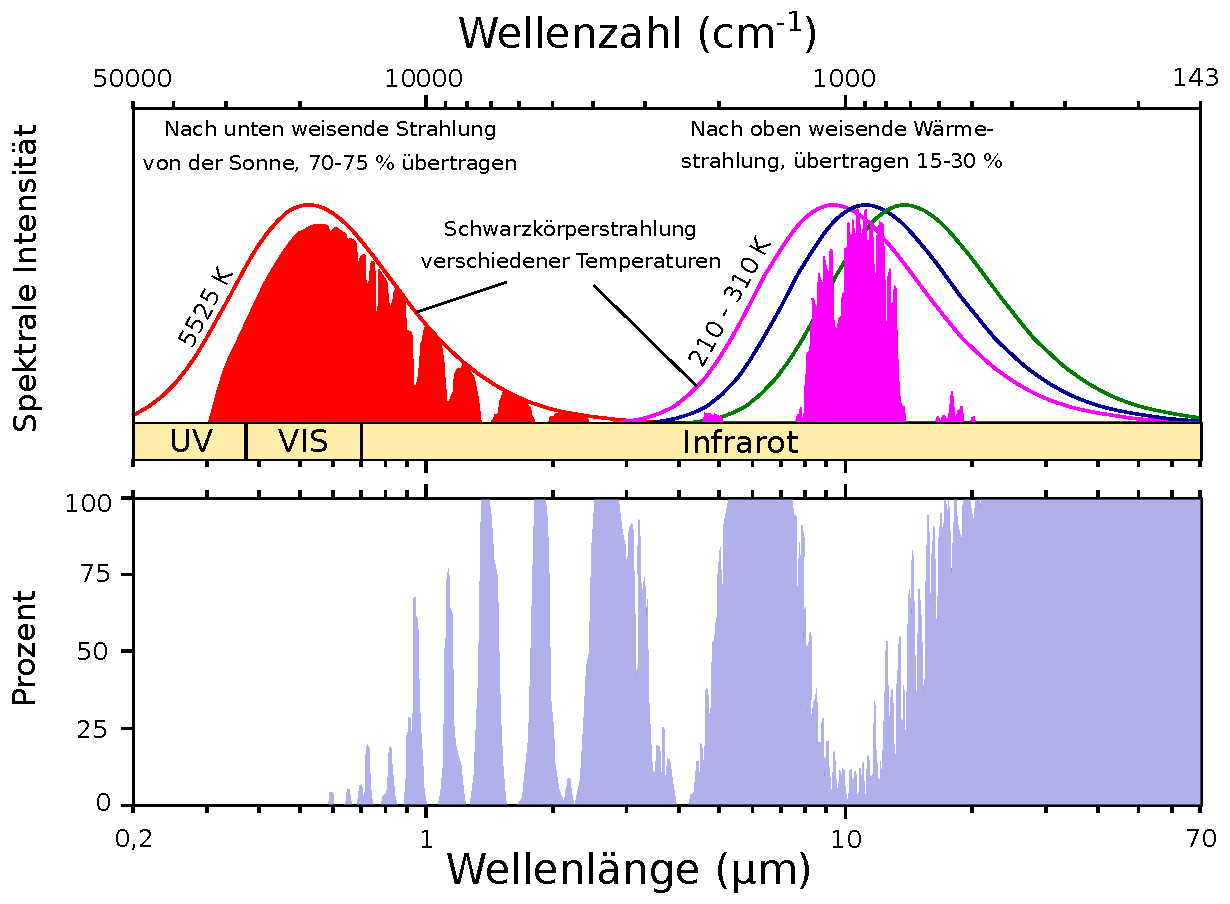
\includegraphics[width=0.7\linewidth]{bilder/Atmospheric_Transmission-H2O.pdf}
    }
    \only<2>{
  	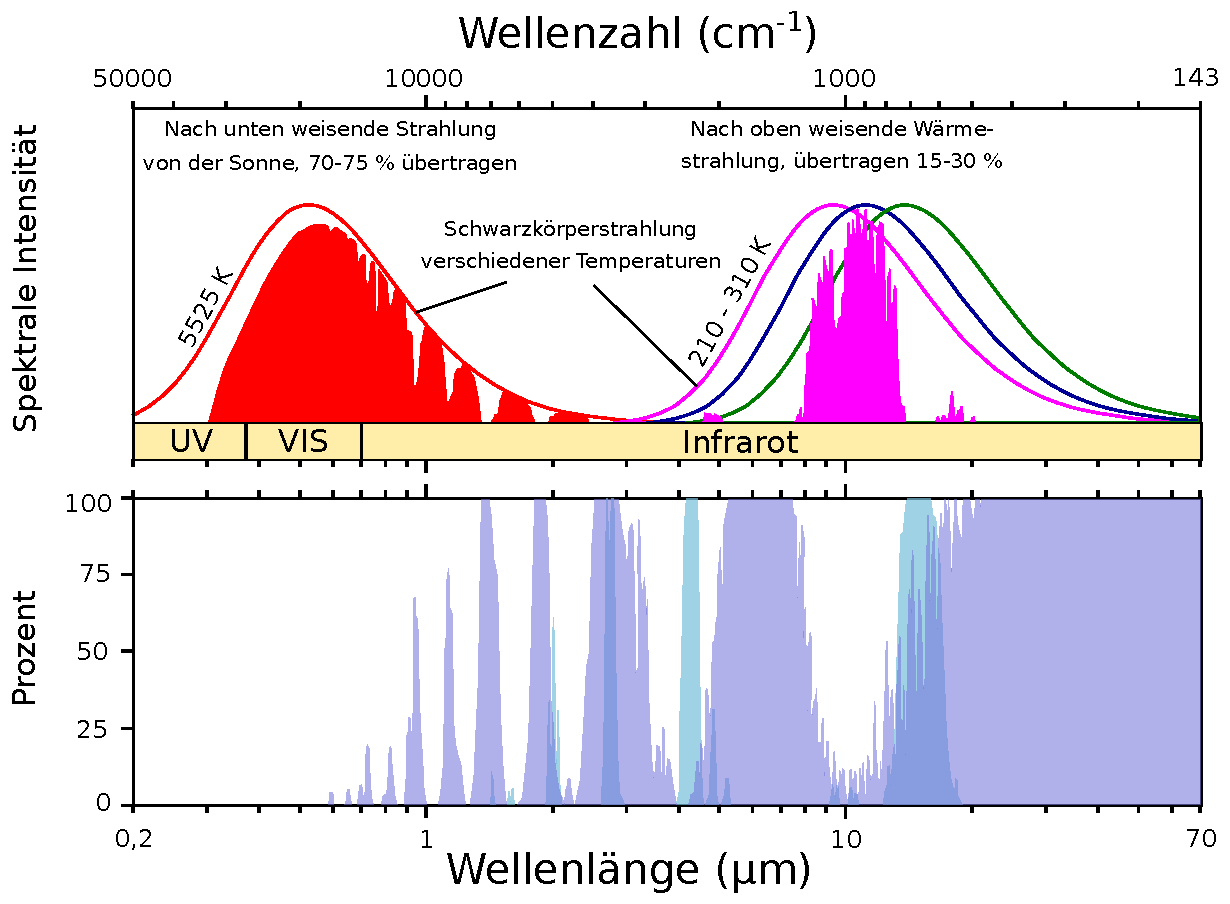
\includegraphics[width=0.7\linewidth]{bilder/Atmospheric_Transmission-H2O-CO2.pdf}
    }
    \only<3>{
  	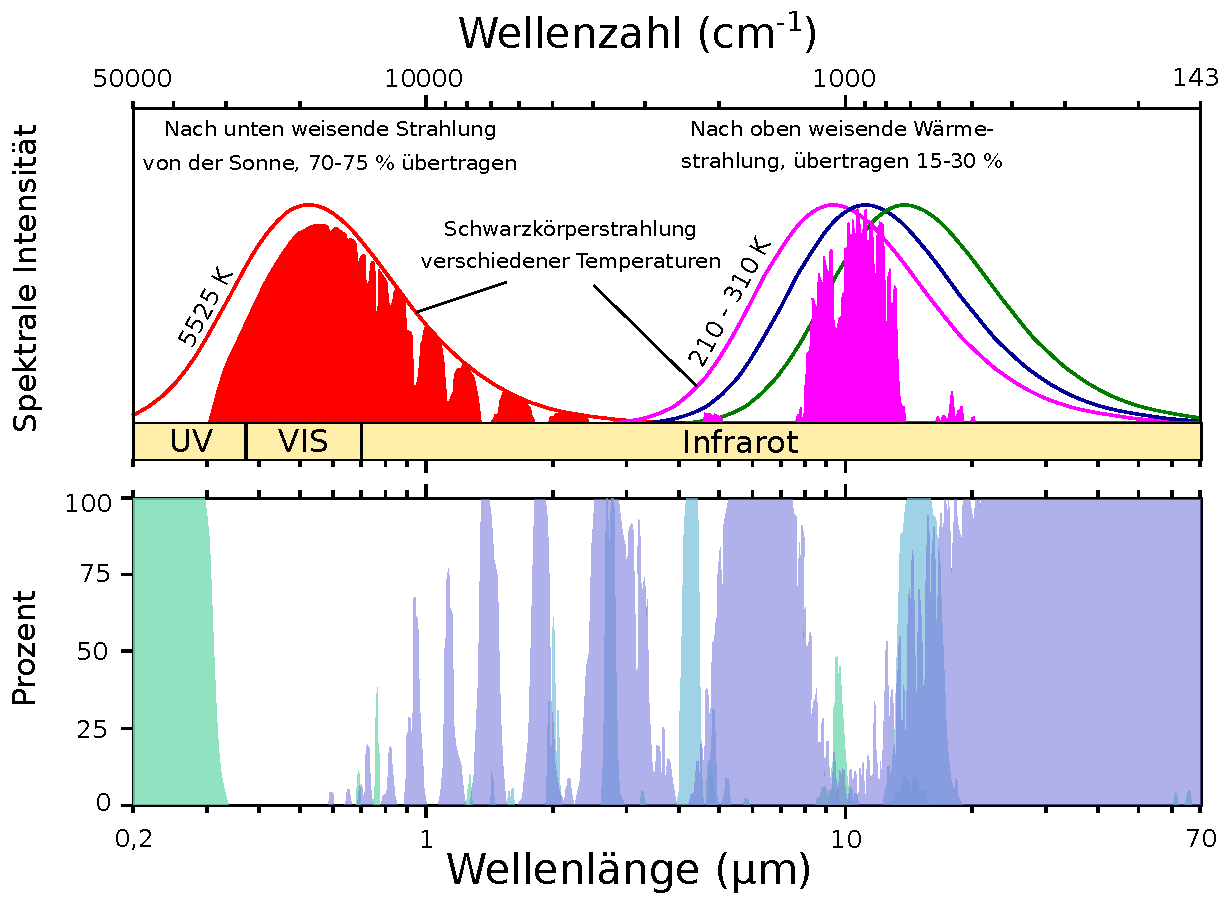
\includegraphics[width=0.7\linewidth]{bilder/Atmospheric_Transmission-H2O-CO2-O2O3.pdf}
    }
    \only<4>{
  	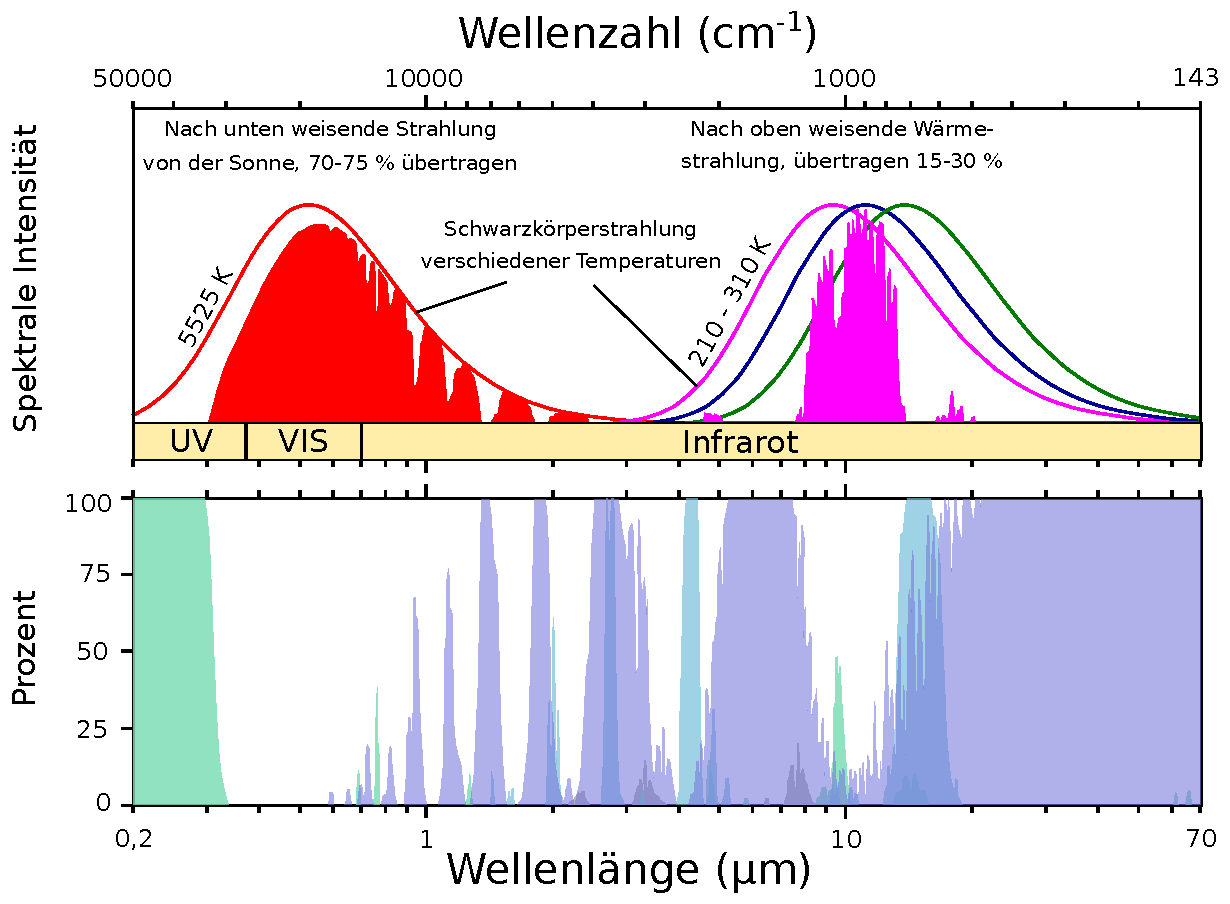
\includegraphics[width=0.7\linewidth]{bilder/Atmospheric_Transmission-H2O-CO2-O2O3-CH4.pdf}
    }
    \only<5>{
  	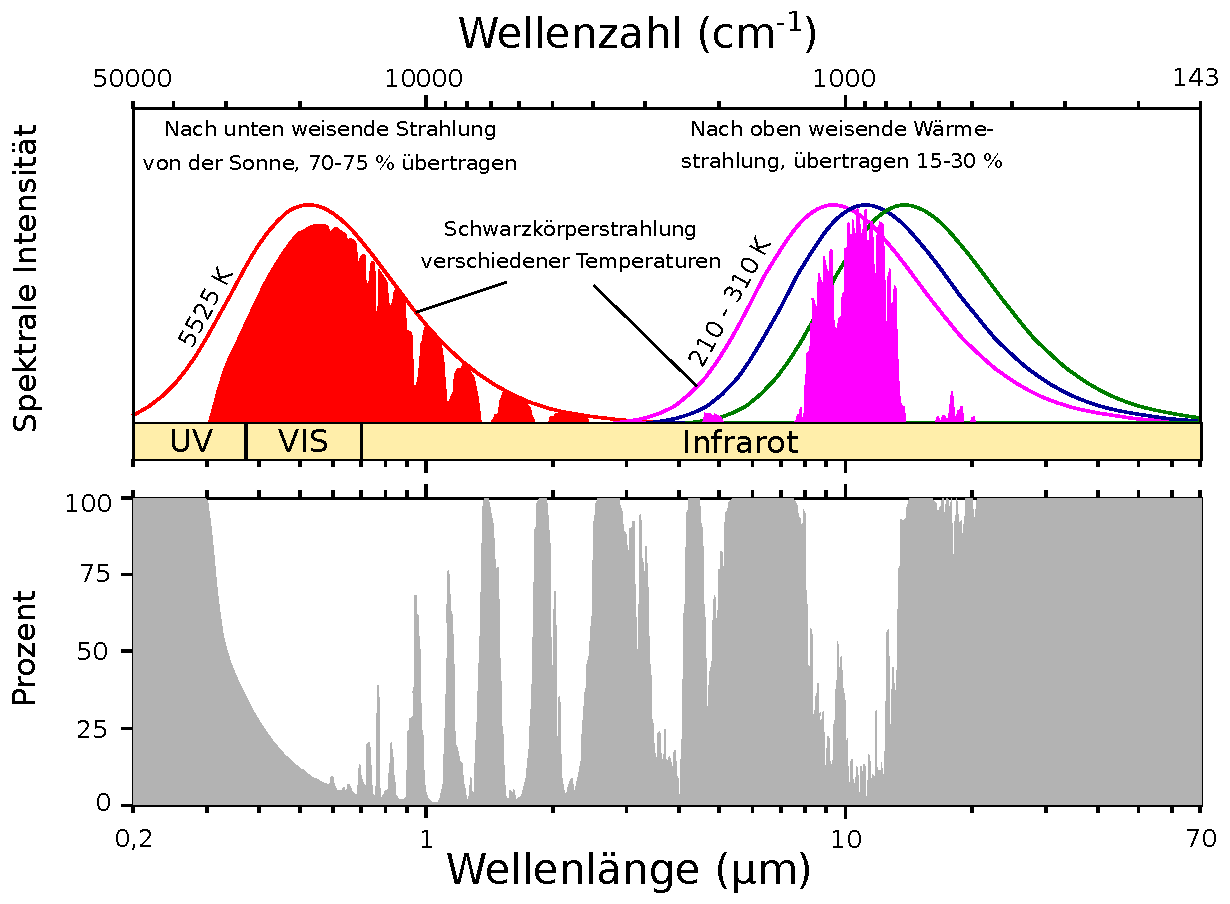
\includegraphics[width=0.7\linewidth]{bilder/Atmospheric_Transmission-all.pdf}
    }
  	\caption{Absorption und Streuung der Atmosphäre, Quelle: Robert A. Rohde, Global Warming Art project}
  \end{figure}

  \note{
  \begin{itemize}
    \item[] Thermische Ausstrahlung der Erde etwa \SI{240}{W\per m\squared}
    \item[$\rightarrow$] entspricht einer Strahlungstemperatur von etwa \SI{-20}{°C} (Plancksches Strahlungsgesetz, Wärmestrahlung eines schwarzen Körpers)
    \item[] tatsächlich beobachtete Temperatur aber \SI{35}{°C} höher, Wie ist das möglich?
    \item[]
		\item  {\color{red}{Wasserdampf $H_2O$}} -  großer Teil des natürlicher Treibhauseffekt % Als Brücke von der vorherigen Folie, 60 % des natürlichen Treibhasueffekts lassen sich auf das Vorkommen von Wasserdampf in der Atmosphäre zurückführen
		\item  {\color{red}{Kohlenstoffdioxid $CO_2$}} - entsteht u.A. bei der Nutzung fossiler Brennstoffe (Öl, Kohle, Gas)
    \item[$\rightarrow$] Anstieg auf den Menschen zurückzuführen
    \item  {\color{red}{Ozon $O_3$}} - entsteht bei Reaktion von Auto-Abgasen in der Luft im Sonnenlicht
		\item  {\color{red}{Methan $CH_4$}} - entsteht u.a. bei der Zersetzung von organischem Material
		\item[$\rightarrow$] $>$ 60\,\% der globalen Methan-Emissionen sind auf menschliche Aktivitäten zurückzuführen %ClimateChange Kurs der Uni Helsinki Chapter 1.3.3
		\item  {\color{red}{Distickstoffmonoxid $N_2O$ (Lachgas)}} - entsteht beim Abbau von Düngemitteln in der Erde
		\item {\color{red}{fluorierte Treibhausgase (F-Gase)}}
		\item[$\rightarrow$] kommen nicht natürlich vor, sehr treibhauswirksam, verweilen z.T. sehr lange in der Atmosphäre, % bis zu 10.000 Jahre
		aber kommen nur in sehr geringer Konzentration vor

		% lfu bayern
		% Zu den F-Gasen zählen die voll halogenierten Fluorkohlenwasserstoffe (FKW, englisch: PFC), die teilhalogenierten Fluorkohlenwasserstoffe (HFKW, englisch: HFC), Schwefelhexafluorid (SF6) und Stickstofftrifluorid (NF3).
		% F-Gase kommen in der Natur nicht vor; aber befinden sich u.a. in Gefriertruhen, Klimaanlagen, Feuerlöschern und Dämmstoffen.
	\end{itemize}
  }
\end{frame}

\begin{frame}
	\frametitle{Treibhausgase} % TODO: Folie evtl. rausnehmen, da zu unübersichtlich

	% TODO: Ist das zu unübersichtlich? Der Fokus soll auf der Verweildauer und dem EInfluss auf den Treibhauseffekt liegen --> evtl Informationen entfernen


	% Werte für CO2, CH4, und N2O von WMO GREENHOUSE GAS BULLETIN No. 15 | 25 November 2019
	% Tabelle von: https://wiki.bildungsserver.de/klimawandel/index.php/Treibhausgase#cite_note-4
	% RF bom Annual Greenhouse Gas index 2018

	% ppm steht für parts per million
	\begin{tabular}{p{2.5cm}|p{3cm}|p{3cm}|p{2cm}|p{2cm}}
		Treibhausgas & Konzentration in der Atmosphäre (2018) & mittlerer jährlicher absoluter Anstieg (2008-2018) & mittlere Verweil-dauer in der Atmosphäre [Jahre] & Strahlungs-antrieb (Radiative Forcing) \\ \\
		\hline
		Kohlenstoff-dioxid ($CO_2$) & (407,8 $\pm$ 0,1) $ppm$ & 2,26 $ppm$\,$y^{-1}$ &  30-1000 & $\approx$ \SI{2}{\watt\per\square\metre} \\
		\hline
		Methan ($CH_4$) & (1869 $\pm$ 2) $ppb$ & 7,1 $ppb$\,$y^{-1}$ &9,1 & $\approx $ \SI{0,5}{\watt\per\square\metre}  \\
		\hline
		Lachgas ($N_2O$) & (331,1 $\pm$ 0,1) $ppb$ & 0,95 $ppm$\,$y^{-1}$ & 131 & $\approx $ \SI{0,2}{\watt\per\square\metre}  \\
	\end{tabular}
	Es gibt noch weitere Treibhausgase, die hier aufgelisteten sind die wichtigsten für den anthropogenen Treibhauseffekt.

\end{frame}


\begin{frame}
	\frametitle{Treibhausgase}
	\begin{figure}
		\centering
		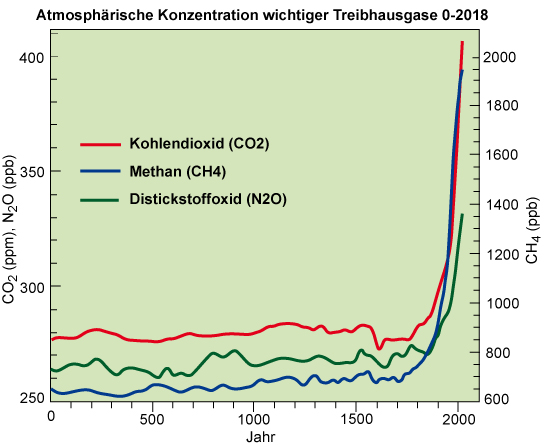
\includegraphics[width=0.6\linewidth]{bilder/Treibhausgase0-aktuell_bildungsserver_hh.jpg}
		\caption{Treibhausgaskonzentration in der Atmosphäre, Quelle: Bildungsserver Hamburg}
		%Abbildung wie in S.Ranmstorf S.33 -> http://www.pik-potsdam.de/~stefan/Publications/Book_chapters/Der_Klimawandel_Kapitel2.pdf oder direkt im IPCC 2013: https://www.ipcc.ch/report/ar5/wg1/observations-atmosphere-and-surface/ Fig 2.1-2.3
	\end{figure}
\end{frame}



\begin{frame}
	\frametitle{Treibhausgase - Klimawirksamkeit}
	\begin{figure}
		\begin{figure}
			\begin{columns}
				\column{0.6\linewidth}
				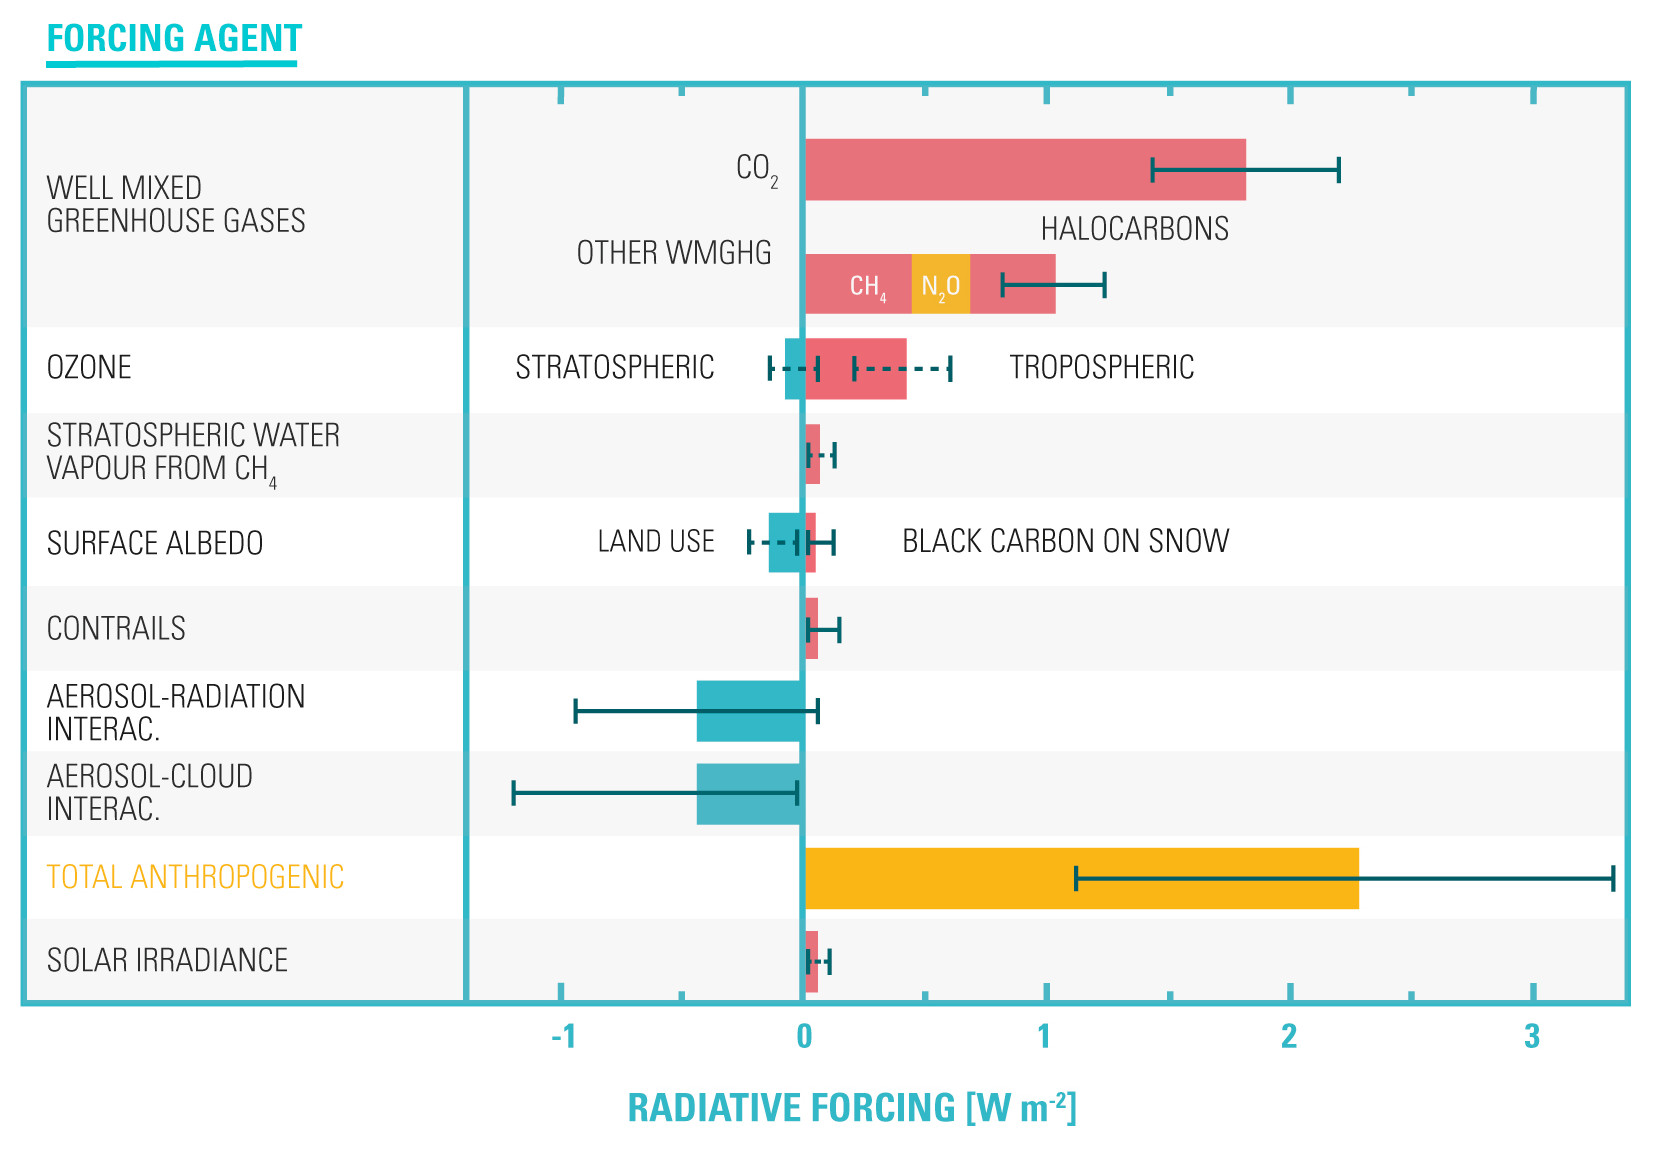
\includegraphics[width=0.9\linewidth]{bilder/radiative_forcing_CCnow_mooc.jpg}
				\column{0.3\linewidth}
				\caption{Strahlungsantrieb der Treibhausgase zwischen 1750 und 2011, Quelle: Climate.now MOOC, abgewandelt von IPCC 2014 Kapitel 8}
			\end{columns}
		\end{figure}
	\end{figure}
\begin{itemize}
	\item Die Änderungen des Strahlungsantriebs sind durch den Menschen verursacht (ersichtlich durch den betrachten Zeitraum)
	\item $CO_2$, $CH_4$ und $N_2O$ zählen zu den langlebigen Treibhausgasen und sind über den Globus verteilt.
	\item Der Grad des wissenschaftlichen Verständnis über diese ist hoch!
	% O3 ist kontinental bis global verbereitet und das Verständnis ist Mittel
	% CH4 ist global verbreitet jedoch ist das Versändnis über den Strahlungsantrieb gering.
	% Das Verständnis sinkt nach Einträgen und daher besonders für die verringernden RF-Faktoren wie Albedo ungewiss. Die Verringerung könnte auch deutlich niedriger liegen, was bedeutet, dass der von den Menschen verursachte Strahlungsantireb sogar noch stärker ist. - Da durch die Erderwärmung und Rußablagerungen auf dem Eis der Albedo-Effekt geschmälert wird, ist das sogar wahrscheinlich.
	% Ergänzungen aus der Abbildung: https://wiki.bildungsserver.de/klimawandel/index.php/Strahlungsantrieb
\end{itemize}
\end{frame}


\begin{frame}
	\frametitle{$CO_2$-Äquivalent}

	\begin{block}{Strahlungsantrieb / Radiative Forcing / RF}
		Strahlungsenergie pro Sekunde und pro Quadratmeter, die durch die Tropopause hindurch kommt \\
		Einheit: %\SI{}{\joule\per\second\per\square\metre} bzw. %\SI{}{\watt\per\square\meter}
	\end{block}

	\begin{block}{$CO_2$-Äquivalent}
		Integral des RF eines Treibhausgases über einen bestimmten Zeitraum (meist 100 Jahre) im Verhältnis zu dem von $CO_2$

%		Beitrag eines Treibhausgases zum Treibhauseffekt über 100 Jahre gemessen am Beitrag des $CO_2$
	\end{block}


	\color{gray}\rule{\linewidth}{1pt}

	\color{black}

	2018 lag der Wert an $CO_2$-Äquivalenten in der Atmosphäre bei 496 ppm (RF: 3,101)\\
	\textit{zum Vergleich: } 1990 waren es noch 417 ppm (RF: 2,165)\\
	$\rightarrow$ \color{red}{Zuwachs des Strahlungsantriebs um 43 \% seit 1990}
\end{frame}

\begin{frame}
	\frametitle{Klimawirksamkeit der Treibhausgase}
	\begin{itemize}
		\item Methan ($CH_4$) ist ca. 30-mal klimawirksamer als $CO_2$
		\item Lachgas ($N_2O$) ist 265-mal klimawirksamer als $CO_2$
		% das heißt selbst die deutlich kleinere Menge von ihnen in der Atmosphäre (ppb anstatt ppm) hat einen deutlichen Einfluss
	\end{itemize}
%(Quelle: IPCC 2014, Kapitel 8, Tabelle 8.7) %Treibhauswirksamkeit über 100 Jahre ohne Einbezug der Feedbacks - GWP [..] with and without inclusion of climate–carbon feedbacks (cc fb) in response to emissions of the indicated non-CO2 gases

%TODO Abbildung evtl vereinfachen oder bessere Abbildung finden! Einfluss von SO_2 noch nicht betrachtet und generell zu voiele Infos über andere Gase enthalten
% SO_2 könnte Debatte eröffnen, die wir an der Stelle noch nicht führen können
% z.B. Abbildung über Verweildauer in der Atmosphäre IPCC 2014 Kapitel 8 Anhang 8.A
	\begin{columns}
	\column{0.5\linewidth}
		\begin{figure}
			\centering
			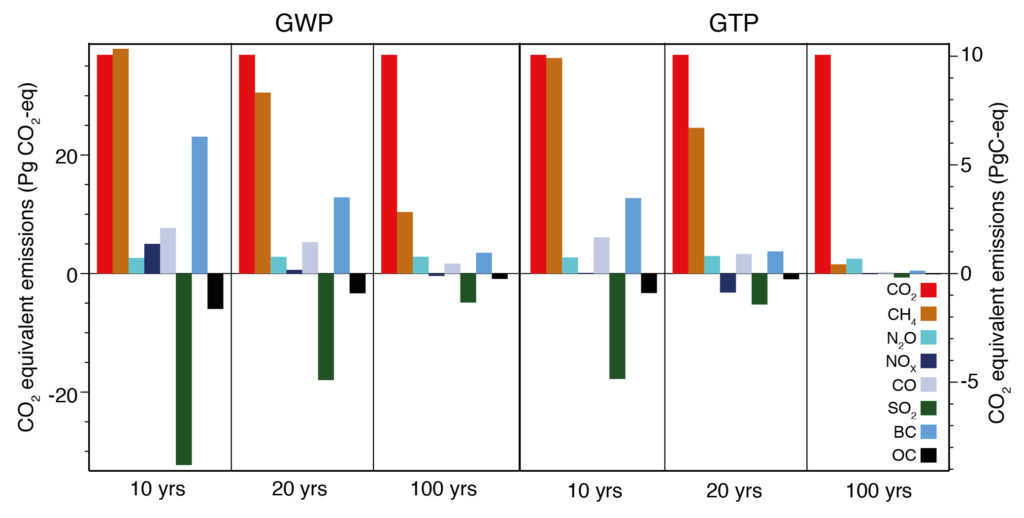
\includegraphics[width=\linewidth]{bilder/IPCC_GWP_anthropogenic_emissions.jpg}
			\caption{Globale von Menschen verursachte Emissionen sortiert nach Klimawirksamkeit (GWP), Quelle: IPCC 2014, Kapitel 8}
		\end{figure}
		\column{0.5\linewidth}
		$\rightarrow$ $CO_2$, $CH_4$ und $N_2O$ haben über die Zeit die höchste Klimawirksamkeit\\
		$\rightarrow$ $CO_2$ verliert über den Zeitraum von 100 Jahren kaum an Klimawirksamkeit\\
%		auch Methan bleibt vergleichsweise lange klimawirksam\\
	\end{columns}
\end{frame}

\begin{frame}
	\frametitle{Eis-Albedo-Rückkopplung}%Rahmstorf, Schellnhuber - Der Klimawandel S. 14
	 Reflexion der ankommenden Sonneneinstrahlung durch Eismassen

	 \begin{columns}[T] % align columns
	 	\begin{column}{.48\textwidth}
	 		\centering
	 		\textbf{Abkühlung}\\
	 		\color{blue}\rule{\linewidth}{4pt}
	 		\color{black}
	 		\color<2->{gray}
	 		je mehr Eismassen\\
	 		$\downarrow$\\
	 		desto mehr wird reflektiert/\\
	 		desto weniger wird absorbiert\\
	 		$\downarrow$\\
	 		desto kälter wird es auf dem Planeten\\
	 		$\downarrow$\\
	 		desto weniger Wasserdampf kann die Atmosphäre aufnehmen\\
	 		$\downarrow$\\
	 		desto geringer wird der Treibhauseffekt
	 	\end{column}%
	 	\hfill%
	 	\begin{column}{.48\textwidth}<2->
	 		\centering
	 		\textbf{Aufwärmung}\\
	 		\color{red}\rule{\linewidth}{4pt}
	 		\color{black}
	 		je weniger Eismassen\\
	 		$\downarrow$\\
	 		desto weniger wird reflektiert/\\
	 		desto mehr wird absorbiert\\
	 		$\downarrow$\\
	 		desto wärmer wird es auf dem Planeten\\
	 		$\downarrow$\\
	 		desto mehr Wasserdampf kann die Atmosphäre aufnehmen\\
	 		$\downarrow$\\
	 		desto stärker wird der Treibhauseffekt
	 	\end{column}%
	 \end{columns}


\end{frame}

% "Runterscrollen" / "Zoom" in einer Abbildung von den Atmosphärischen Schichten auf die Erde
